\documentclass[aspectratio=169,10pt]{beamer}
\usetheme{default}
\usecolortheme{default}
\setbeamertemplate{navigation symbols}{}
\setbeamertemplate{footline}[frame number]
\definecolor{epic}{RGB}{20,60,120}
\setbeamercolor{frametitle}{fg=epic}
\setbeamercolor{title}{fg=epic}
\setbeamercolor{structure}{fg=epic}
\setbeamerfont{frametitle}{size=\large,series=\bfseries}
\usepackage{booktabs}
\usepackage{amsmath,amssymb}
\usepackage{graphicx}
\graphicspath{{../../results/}}
\newcommand{\code}[1]{\texttt{\detokenize{#1}}}
\newcommand{\good}[1]{\textcolor{green!45!black}{#1}}
\newcommand{\bad}[1]{\textcolor{red!70!black}{#1}}

\title{$\Lambda\to p\pi^-$ in the ePIC B0 tracker}
\subtitle{Acceptance, tracking efficiency and the reconstructed $\Lambda$ mass\\
old B0 geometry vs eic/epic\#1194}
\author{Gadi Ninio}
\date{3 November 2026}

\begin{document}

\begin{frame}
\titlepage
\centering\footnotesize Code, results, report: \url{https://github.com/gadininio/eic-B0-detector}
\end{frame}

%-------------------------------------------------------------------------------------
\begin{frame}{Introduction and motivation}
\begin{itemize}
\item Far-forward $\Lambda$: production and polarization in the target fragmentation region,
$\Lambda$ tagging in exclusive/diffractive reactions
\item At high energy the $\Lambda$ flies at a few to $\sim$20\,mrad from the proton beam and decays
\textbf{metres downstream}: $c\tau = 7.89$\,cm $\Rightarrow$ $\langle L\rangle \approx 5.3$\,m at 75\,GeV
\item The B0 tracker sits at $z \approx 5.8$--$6.9$\,m, inside the B0 dipole
\item $\Lambda\to p\pi^-$ (64\,\%) must be reconstructed in B0 from tracks that \textbf{do not come from the IP}
\end{itemize}
\vspace{2mm}
\textbf{Goal:} reconstruct the $\Lambda$ mass from B0 tracks, step by step, and understand each loss:
\begin{itemize}
\item acceptance (what the detector covers) $\to$ tracking efficiency $\to$ acceptance $\times$ efficiency $\to$ mass
\item compare the B0 geometry of the nightly with the realistic B0 of \textbf{eic/epic\#1194}
\end{itemize}
\end{frame}

%-------------------------------------------------------------------------------------
\begin{frame}{Setup}
\begin{columns}[T]
\column{0.5\textwidth}
\textbf{Sample} (single-$\Lambda$ gun)
\begin{itemize}\small
\item $p = 50$--$100$\,GeV, $\theta = 8$--$18$\,mrad, $\phi$ uniform
\item 25\,mrad crossing angle, 18$\times$275 craterlake
\item 100 ev.\ (seed 42), \textbf{1000 ev.}\ (2$\times$500) per geometry
\item 5000 geantinos per geometry
\end{itemize}
\textbf{Composition} (1000 ev.)
\begin{itemize}\small
\item $\Lambda\to p\pi^-$ 48--50\,\%, $n\pi^0$ 25--28\,\%, other 24--25\,\% (interactions)
\item 88--90\,\% of $p\pi^-$ decays before B0
\item $M(p\pi^-)$ from true momenta = 1.115683\,GeV
\end{itemize}
\column{0.5\textwidth}
\textbf{Software}
\begin{itemize}\small
\item ddsim in eic-shell (nightly)
\item \textbf{old} geometry: epic \code{43f427e}, sensors 300\,$\mu$m
\item \textbf{new} geometry: epic main \code{ec774d8} (\#1194), sensors 50\,$\mu$m
\item EICrecon main \code{8b44cae} (with \#2901)
\item ACTS CKF with \textbf{truth seeding}
\end{itemize}
\end{columns}
\end{frame}

%-------------------------------------------------------------------------------------
\begin{frame}{Definitions}
\small
\begin{tabular}{@{}p{0.27\textwidth}p{0.68\textwidth}@{}}
\toprule
$\Lambda\to p\pi^-$ decay & generated $\Lambda$ with exactly two daughters, $p$ and $\pi^-$ \\
Accepted daughter & its own \emph{simulated} B0 hits cover $\ge 3$ layers (enough for a track)\\
Reconstructed daughter & a reconstructed particle whose best truth match is the daughter\\
\midrule
\textbf{Geometric acceptance} & straight lines from the IP at the $\Lambda$ angles crossing $\ge 3$ layers (geantinos). \emph{Not} a $\Lambda$ acceptance: the $\Lambda$ is neutral\\
\textbf{Daughter acceptance} $A$ & accepted daughters / $p\pi^-$ decays (decay point, field, material; no detector response)\\
\textbf{Tracking efficiency} $\varepsilon$ & reconstructed accepted daughters / accepted daughters (geometry cancels)\\
\textbf{Acceptance $\times$ efficiency} & reconstructed daughters / $p\pi^-$ decays $= A\cdot\varepsilon$\\
\midrule
Purity & signal / selected candidates (truth only labels)\\
B0 threshold & energy per pixel needed for a hit (EICrecon default 10\,keV)\\
\bottomrule
\end{tabular}
\vspace{1mm}\\
\footnotesize Angles w.r.t.\ the proton beam (crossing-angle rotation undone). Layers: hits more than 50\,mm apart in $z$.
\end{frame}

%-------------------------------------------------------------------------------------
\begin{frame}{First look: only 4 B0 tracks per 100 $\Lambda$}
\begin{itemize}
\item Nightly EICrecon (\code{a7bab3f}): the truth seeder only seeded particles from $|z| < 200$\,mm
$\Rightarrow$ $\Lambda$ daughters from decays metres downstream had \bad{no seed}
\item \textbf{EICrecon\#2901} (in main): dedicated \code{B0TrackerTruthSeeds}, vertex $z < 6$\,m, perigee at the true vertex
\end{itemize}
\vspace{2mm}
\centering
\begin{tabular}{@{}lcc@{}}
\toprule
100 events: nightly $\to$ main & old geometry & new geometry\\
\midrule
B0 reconstructed hits & 1416 & 593\\
truth seeds & 8 $\to$ 650 & 4 $\to$ 504\\
B0 tracks & 4 $\to$ \good{\textbf{77}} & 1 $\to$ \good{\textbf{44}}\\
events with a + and a $-$ track & 1 $\to$ 18 & 0 $\to$ 14\\
\bottomrule
\end{tabular}
\vspace{2mm}
\begin{itemize}
\item Same hits: the whole gain is seeding. Seeds include shower particles $\Rightarrow$ truth matching needed
\end{itemize}
\end{frame}

%-------------------------------------------------------------------------------------
\begin{frame}{Geometric acceptance along the $\Lambda$ direction (geantinos)}
\centering
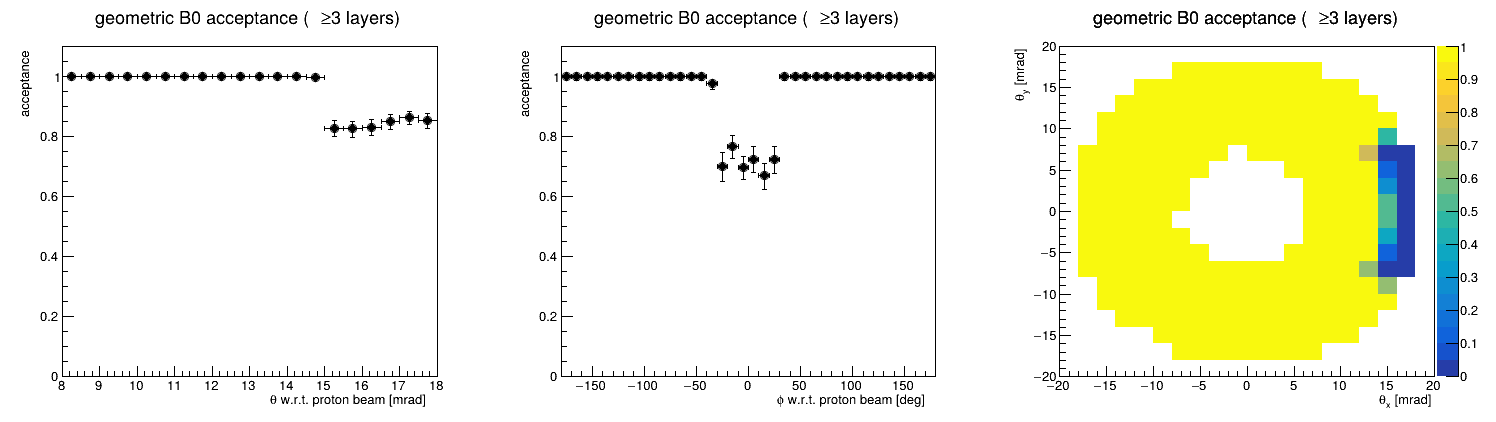
\includegraphics[width=0.75\textwidth]{02_geometric_acceptance/geometric_acceptance_old.png}\\[-1mm]
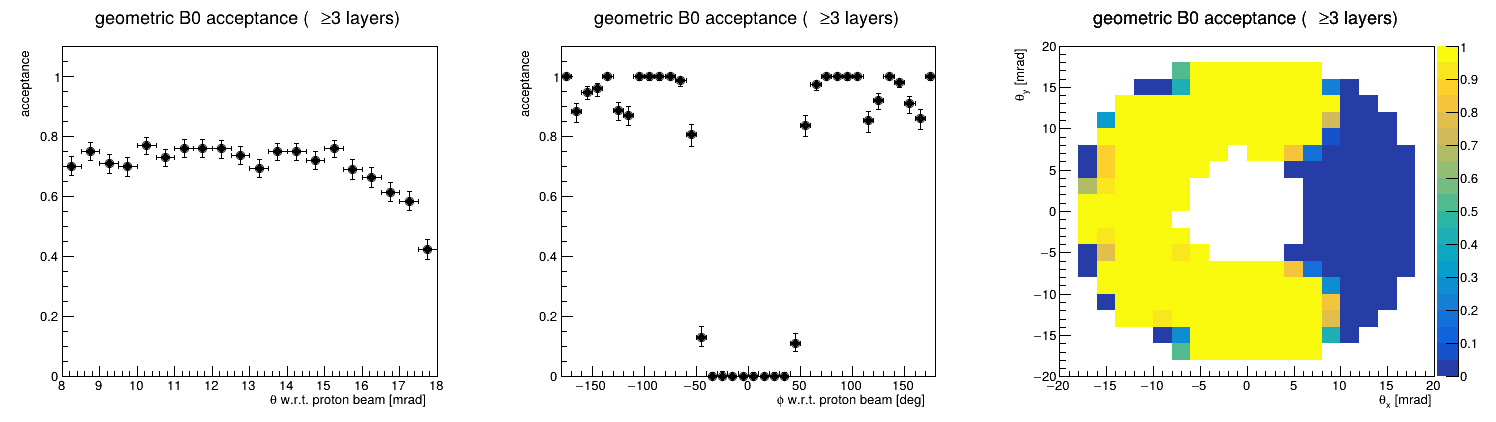
\includegraphics[width=0.75\textwidth]{02_geometric_acceptance/geometric_acceptance_new.png}
\begin{itemize}\small
\item $\ge 3$ layers: \textbf{95.3\,\%} (old, top) vs \bad{\textbf{70.1\,\%}} (new, bottom)
\item New geometry: \textbf{gap of $\pm 45^\circ$ in $\phi$} on the electron-beam side; losses above 16\,mrad
\end{itemize}
\end{frame}

%-------------------------------------------------------------------------------------
\begin{frame}{Decay kinematics: a hard proton and a soft $\pi^-$}
\begin{itemize}
\item $Q = 38$\,MeV: in the $\Lambda$ frame $p^* = 0.101$\,GeV, $E^*_p = 0.943$\,GeV, $E^*_\pi = 0.172$\,GeV
\item Both daughters move with $\approx$ the $\Lambda$ velocity and share its momentum as their rest-frame energies:
\[ \frac{p_p}{p_\Lambda} \in [0.76, 0.94] \;\Rightarrow\; 38\text{--}94\,\text{GeV}, \qquad
   \frac{p_\pi}{p_\Lambda} \in [0.06, 0.25] \;\Rightarrow\; 3\text{--}25\,\text{GeV} \]
\item The soft $\pi^-$ is bent much more by the B0 dipole
\item Momentum ratio, independent of $p_\Lambda$:
\[ r = \frac{p_p}{p_\pi} = \frac{E^*_p + p^*\cos\theta^*}{E^*_\pi - p^*\cos\theta^*} \in [3.09,\ 14.6] \]
(used later for a selection without truth)
\end{itemize}
\end{frame}

%-------------------------------------------------------------------------------------
\begin{frame}{Acceptance for the $\Lambda$ daughters (full simulation, simulated hits)}
\begin{columns}[T]
\column{0.5\textwidth}\centering old geometry\\
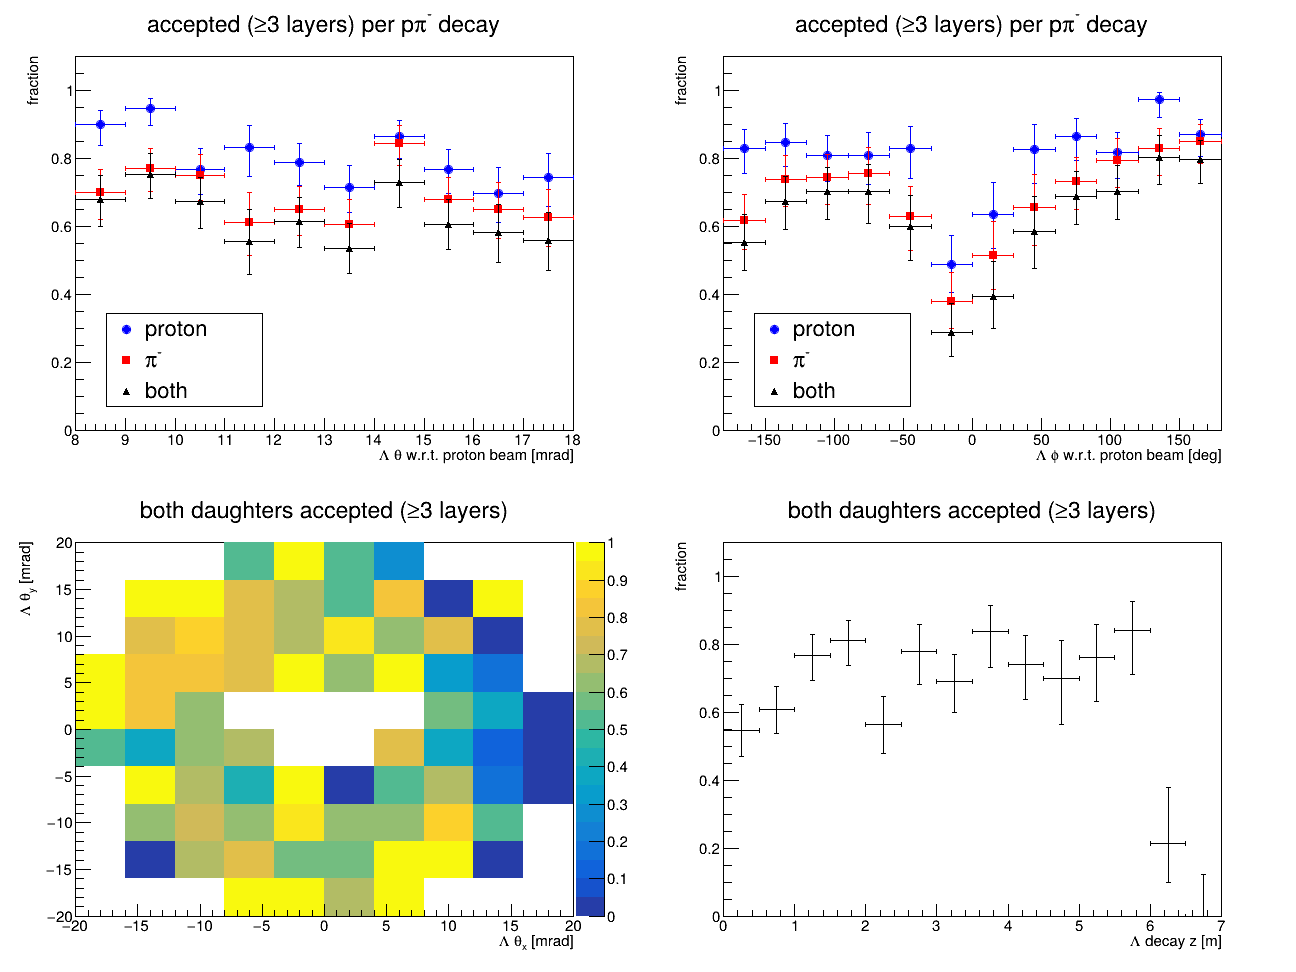
\includegraphics[width=\textwidth]{03_daughter_acceptance/daughter_acceptance_old.png}
\column{0.5\textwidth}\centering new geometry\\
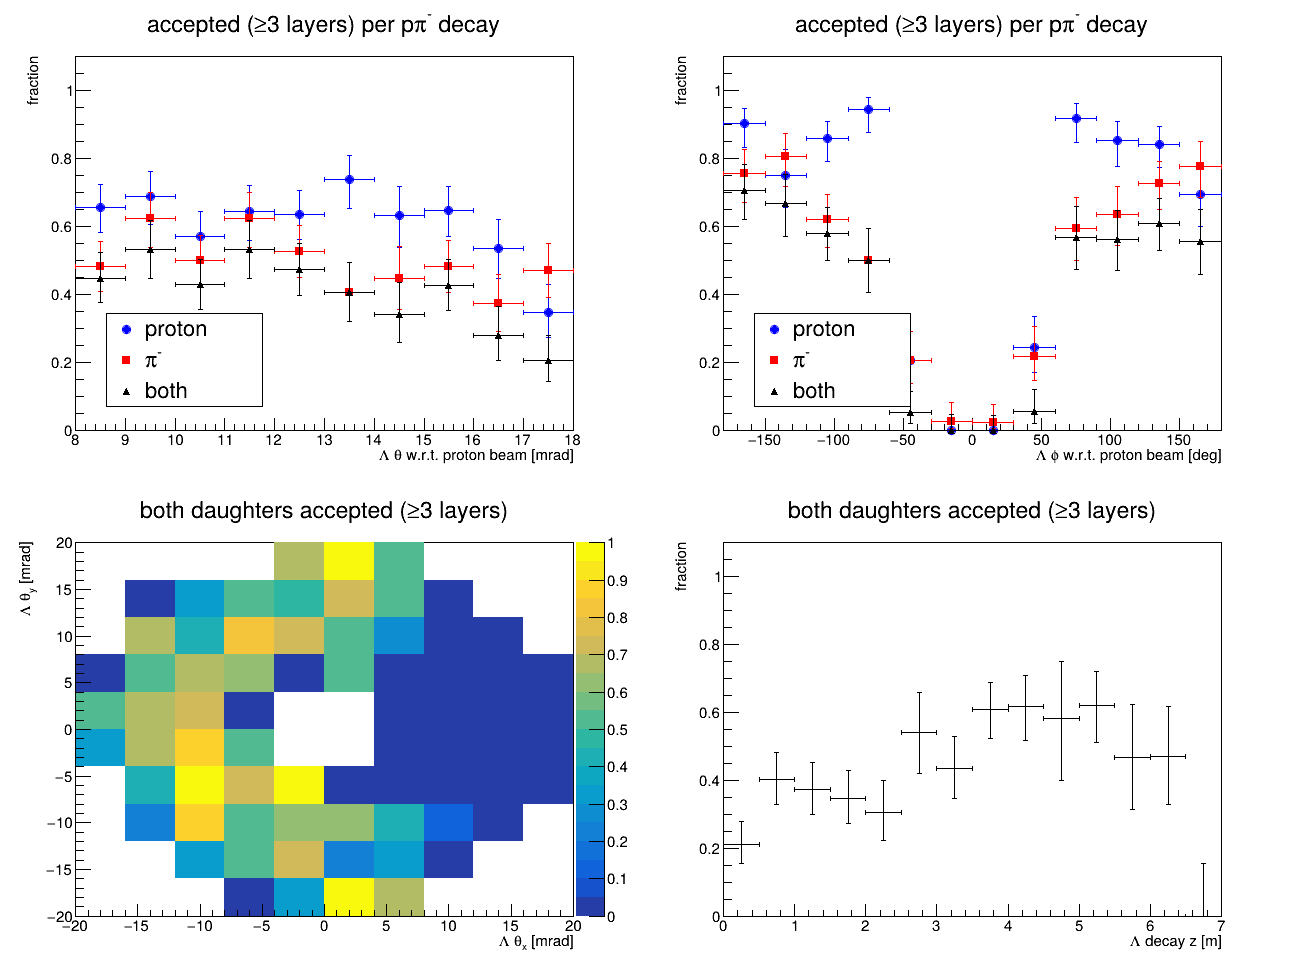
\includegraphics[width=\textwidth]{03_daughter_acceptance/daughter_acceptance_new.png}
\end{columns}
\vspace{1mm}
\small
\begin{tabular}{@{}lccc@{}}
\toprule
per $p\pi^-$ decay, $\ge 3$ layers & proton & $\pi^-$ & \textbf{both}\\
\midrule
old & 80\,\% & 69\,\% & \textbf{63\,\%}\\
new & 61\,\% & 49\,\% & \bad{\textbf{41\,\%}}\\
\bottomrule
\end{tabular}
\hspace{4mm}
\begin{minipage}{0.45\textwidth}\footnotesize
$\approx$ 30 points below the geometric number: decay point, opening angle, $\pi^-$ bending. Rises with the decay distance.
\end{minipage}
\end{frame}

%-------------------------------------------------------------------------------------
\begin{frame}{Tracking efficiency for accepted daughters}
\begin{columns}[T]
\column{0.5\textwidth}\centering old geometry\\
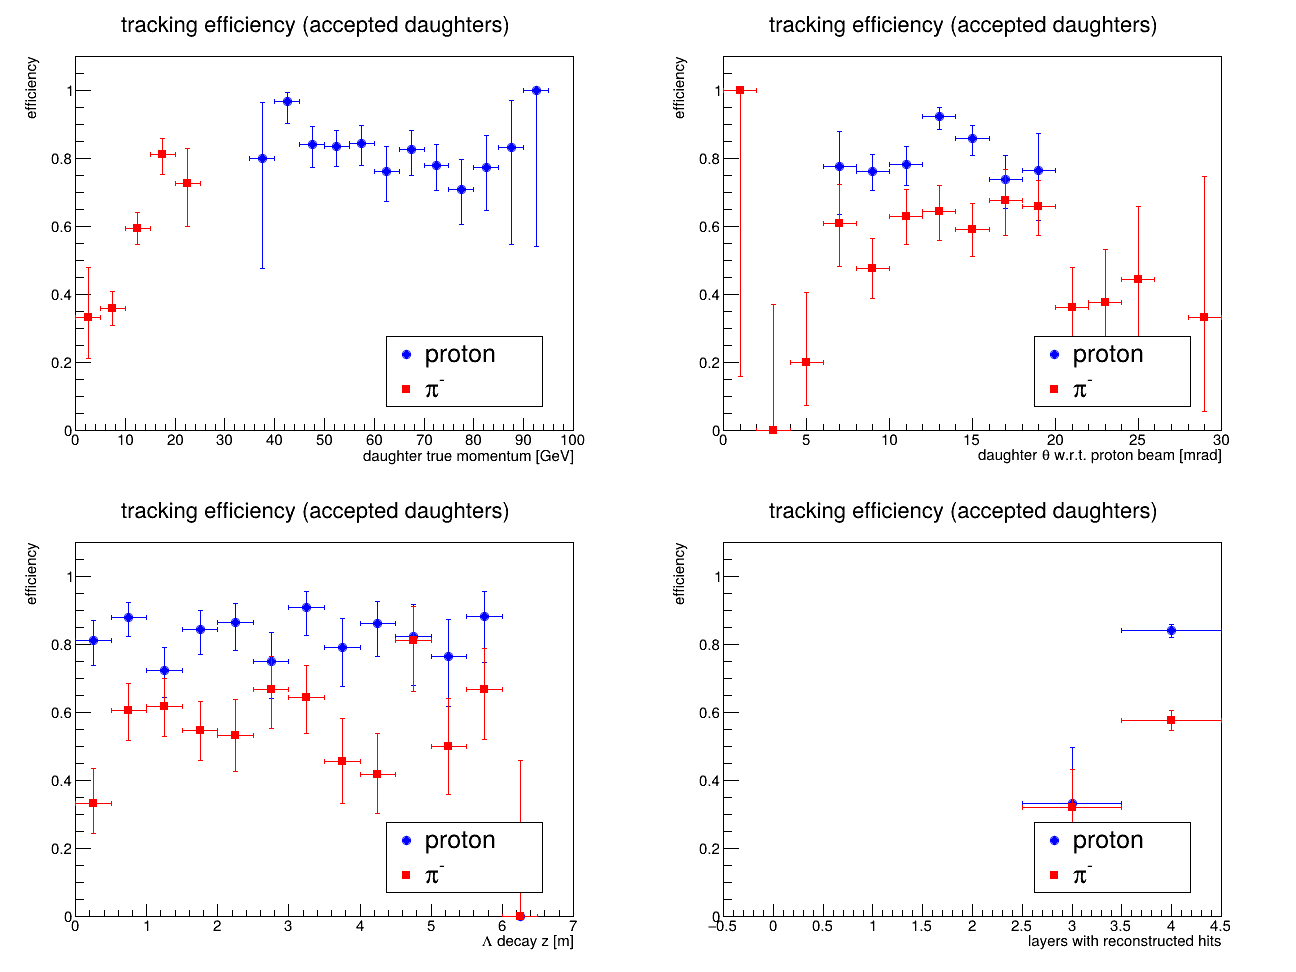
\includegraphics[width=0.92\textwidth]{04_tracking_efficiency/tracking_efficiency_old_10keV.png}
\column{0.5\textwidth}\centering new geometry, 5\,keV\\
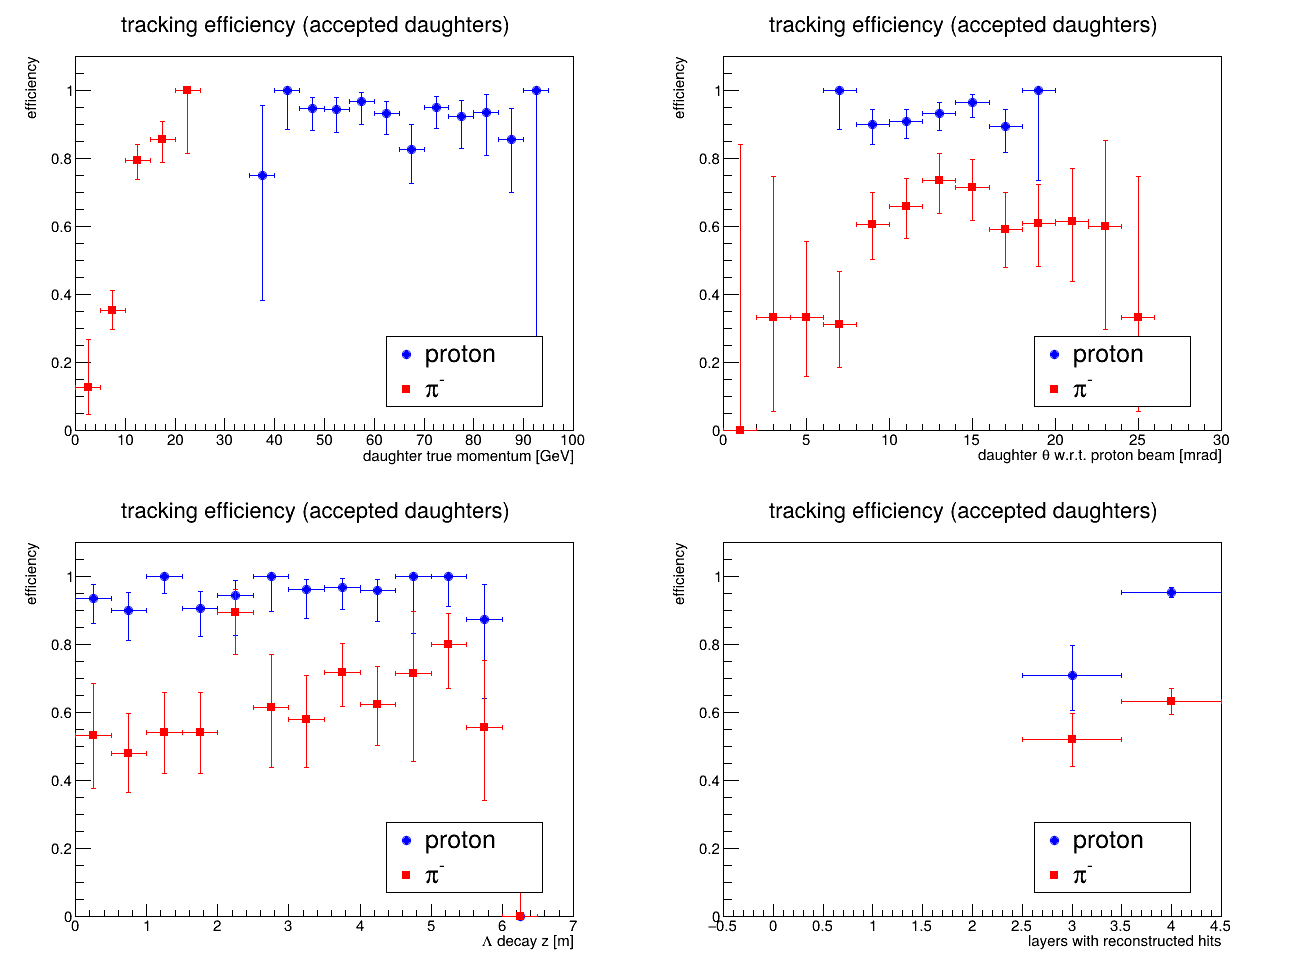
\includegraphics[width=0.92\textwidth]{04_tracking_efficiency/tracking_efficiency_new_5keV.png}
\end{columns}
\small
\begin{itemize}
\item proton 82--93\,\%, $\pi^-$ 56--61\,\%. \textbf{The $\pi^-$ loss is a momentum effect:}
12--36\,\% below 10\,GeV, 75--90\,\% at 10--25\,GeV (as good as the proton)
\end{itemize}
\end{frame}

%-------------------------------------------------------------------------------------
\begin{frame}{Where are the daughters lost?}
\centering\small
\begin{tabular}{@{}lccc@{}}
\toprule
accepted daughters, proton / $\pi^-$ & old & new, 10\,keV & new, 5\,keV\\
\midrule
accepted & 404 / 349 & 295 / 240 & 295 / 240\\
rec.\ hits in $\ge 3$ layers & 100 / 100\,\% & \bad{93 / 93\,\%} & 100 / 100\,\%\\
seed & 99 / 99\,\% & 97 / 96\,\% & 97 / 96\,\%\\
CKF track & \bad{82 / 56\,\%} & \bad{86 / 58\,\%} & \bad{93 / 61\,\%}\\
filtered track & 82 / 56\,\% & 86 / 58\,\% & 93 / 61\,\%\\
reconstructed particle & 82 / 56\,\% & 86 / 58\,\% & 93 / 61\,\%\\
\bottomrule
\end{tabular}
\begin{itemize}
\item Seeds exist; the loss is in the \textbf{CKF} (seed $\to$ track); filtering and particle building lose nothing
\item \textbf{Seed momentum smearing (10\,\%) ruled out:} rerun with \code{MomentumSmear=0} $\Rightarrow$ 71 vs 70 of 120 $\pi^-$
\item Open: CKF $\chi^2$/measurement cuts? multiple scattering? (0,0,0) perigee extrapolation of \#2901?
\end{itemize}
\end{frame}

%-------------------------------------------------------------------------------------
\begin{frame}{The B0 threshold: 50\,$\mu$m sensors need 5\,keV}
\begin{columns}[T]
\column{0.45\textwidth}
\small
\begin{tabular}{@{}lcc@{}}
\toprule
per hit (hadrons) & old & new\\
\midrule
sensor thickness & 300\,$\mu$m & 50\,$\mu$m\\
most probable deposit & 95\,keV & \textbf{13.8\,keV}\\
below 10\,keV & 2.6\,\% & \bad{9.3\,\%}\\
below 5\,keV & 1.6\,\% & 0.3\,\%\\
\bottomrule
\end{tabular}
\vspace{3mm}
\begin{itemize}
\item MIP: $\approx 0.28$\,keV/$\mu$m in Si
\item 10\,keV cuts the Landau tail: 7\,\% of accepted daughters lose layers
\item \good{5\,keV recovers them}; proton eff.\ 86 $\to$ 93\,\%
\item {\scriptsize\code{-PB0TRK:B0TrackerRawHits:threshold=5e-6}}
\item Not the EICrecon default yet
\end{itemize}
\column{0.55\textwidth}\centering
new geometry: 10\,keV (top) / 5\,keV (bottom)\\
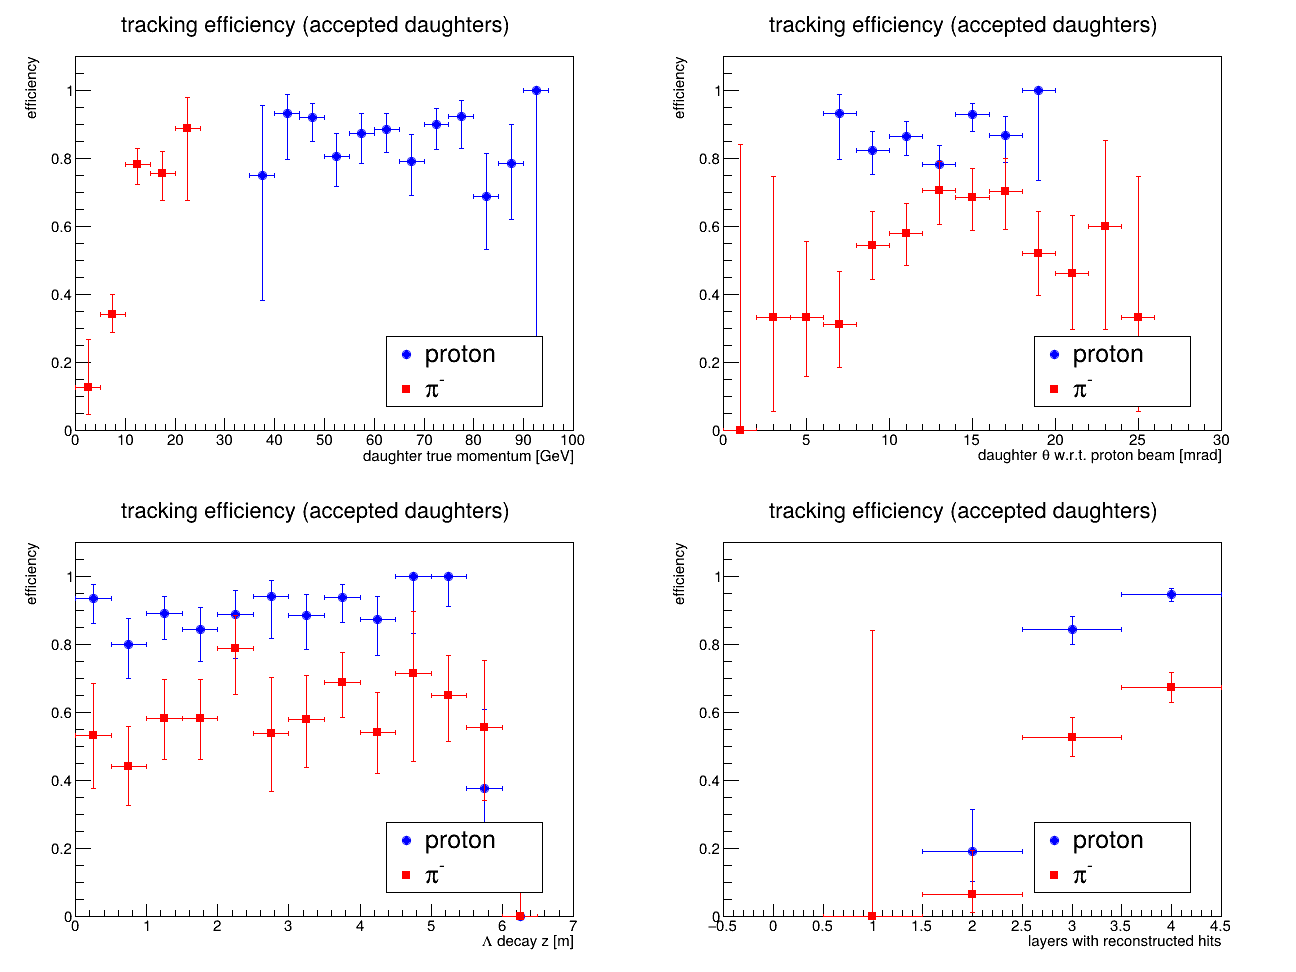
\includegraphics[width=0.62\textwidth]{04_tracking_efficiency/tracking_efficiency_new_10keV.png}\\
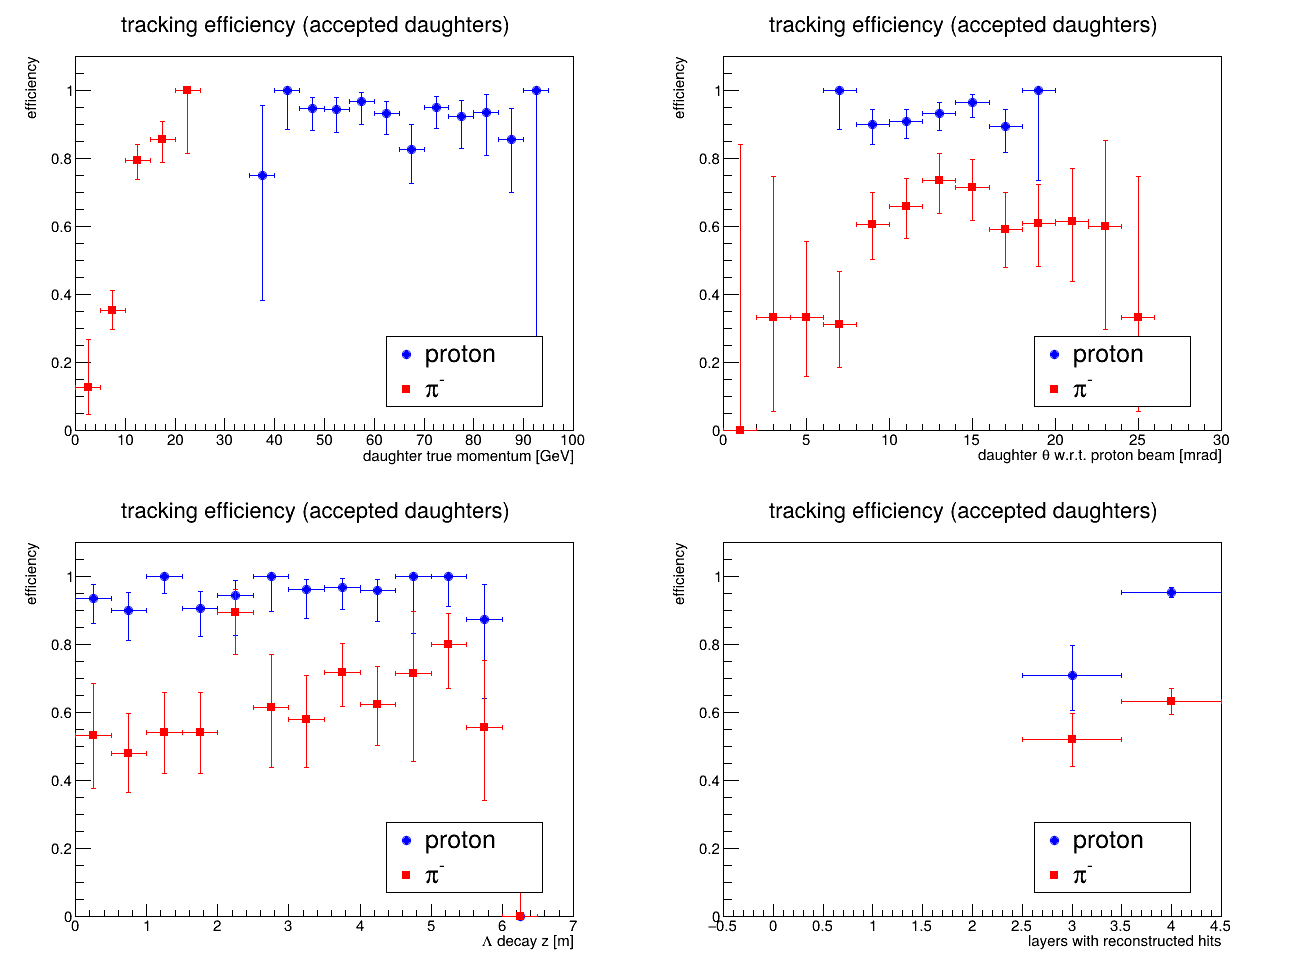
\includegraphics[width=0.62\textwidth]{04_tracking_efficiency/tracking_efficiency_new_5keV.png}
\end{columns}
\end{frame}

%-------------------------------------------------------------------------------------
\begin{frame}{Acceptance $\times$ efficiency}
\begin{columns}[T]
\column{0.5\textwidth}\centering old geometry\\
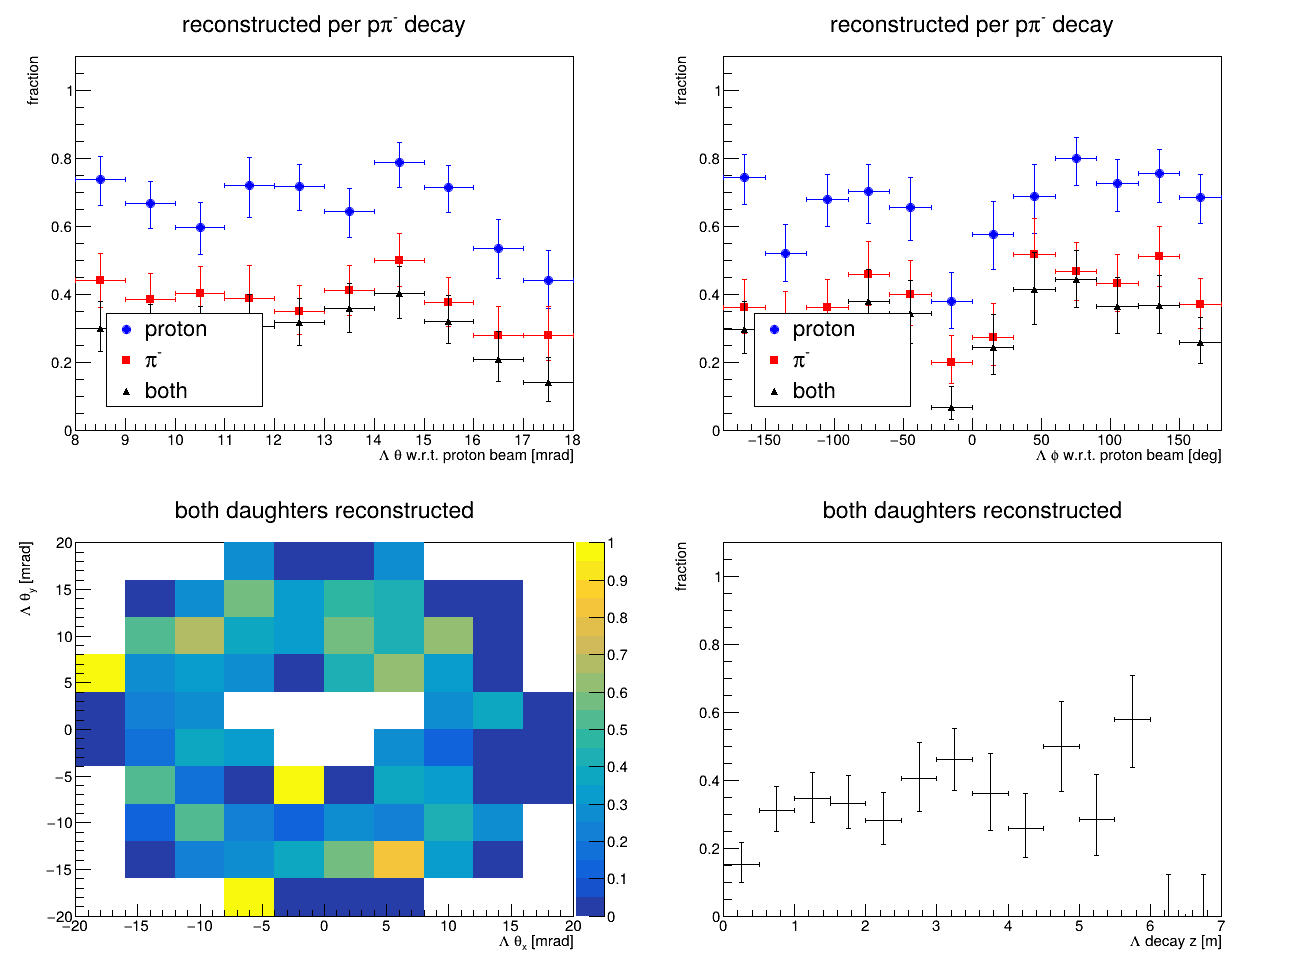
\includegraphics[width=0.9\textwidth]{05_acceptance_x_efficiency/acceptance_x_efficiency_old_10keV.png}
\column{0.5\textwidth}\centering new geometry, 5\,keV\\
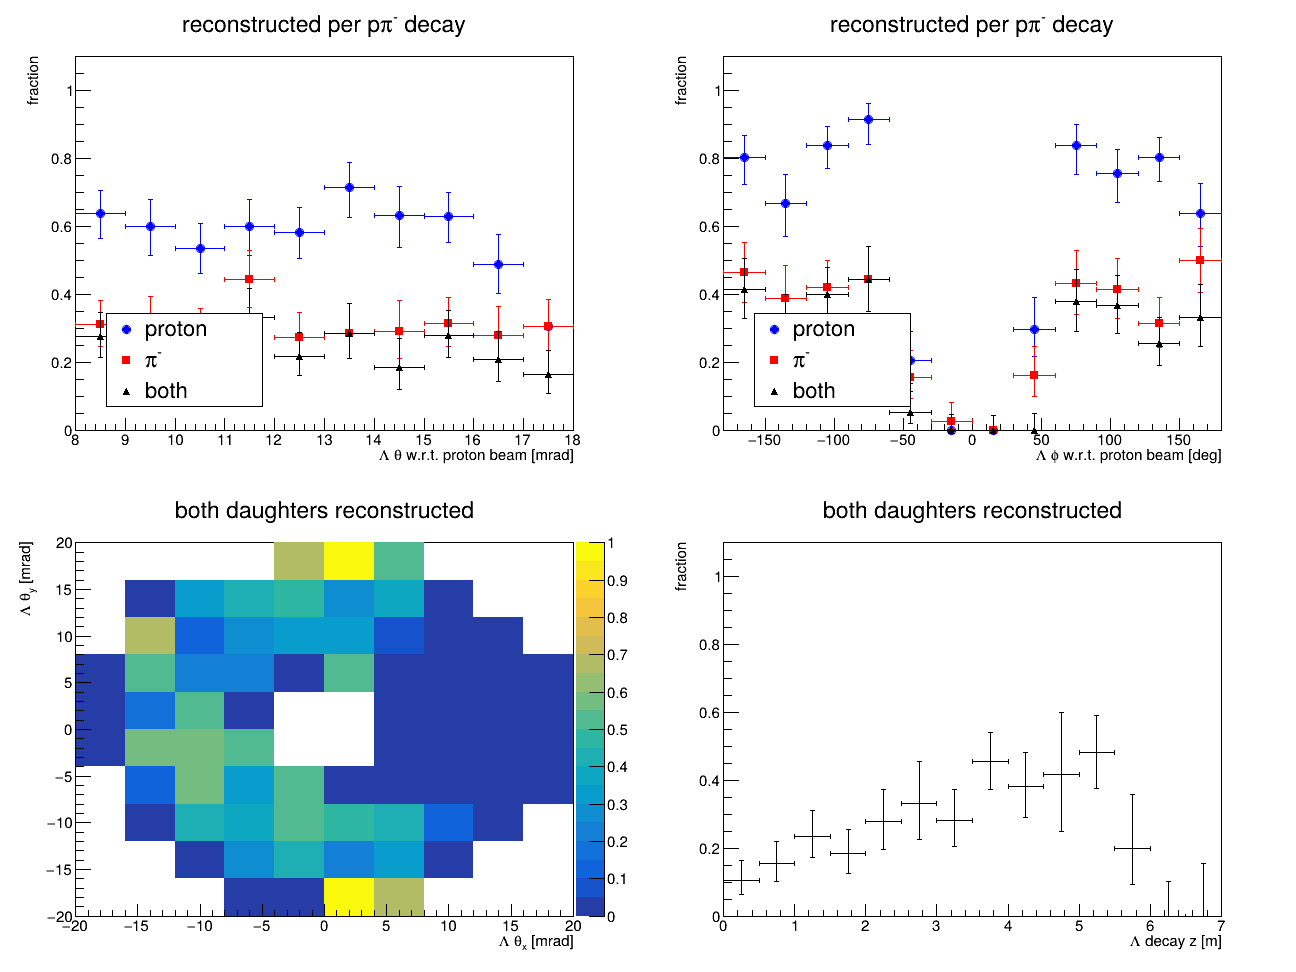
\includegraphics[width=0.9\textwidth]{05_acceptance_x_efficiency/acceptance_x_efficiency_new_5keV.png}
\end{columns}
\centering\small
\begin{tabular}{@{}lccc@{}}
\toprule
proton / $\pi^-$ / both & old & new, 10\,keV & new, 5\,keV\\
\midrule
$A$ & 80 / 69 / 63\,\% & 61 / 49 / 41\,\% & 61 / 49 / 41\,\%\\
$\varepsilon$ & 82 / 56 / 47\,\% & 86 / 58 / 50\,\% & 93 / 61 / 59\,\%\\
$A\times\varepsilon$ & 66 / 39 / \textbf{30\,\%} & 53 / 29 / \textbf{21\,\%} & 57 / 31 / \textbf{25\,\%}\\
per generated $\Lambda$ (both) & \textbf{15.0\,\%} & \textbf{10.1\,\%} & \textbf{12.0\,\%}\\
\bottomrule
\end{tabular}
\end{frame}

%-------------------------------------------------------------------------------------
\begin{frame}{$\Lambda$ mass: truth-matched pairs}
\centering
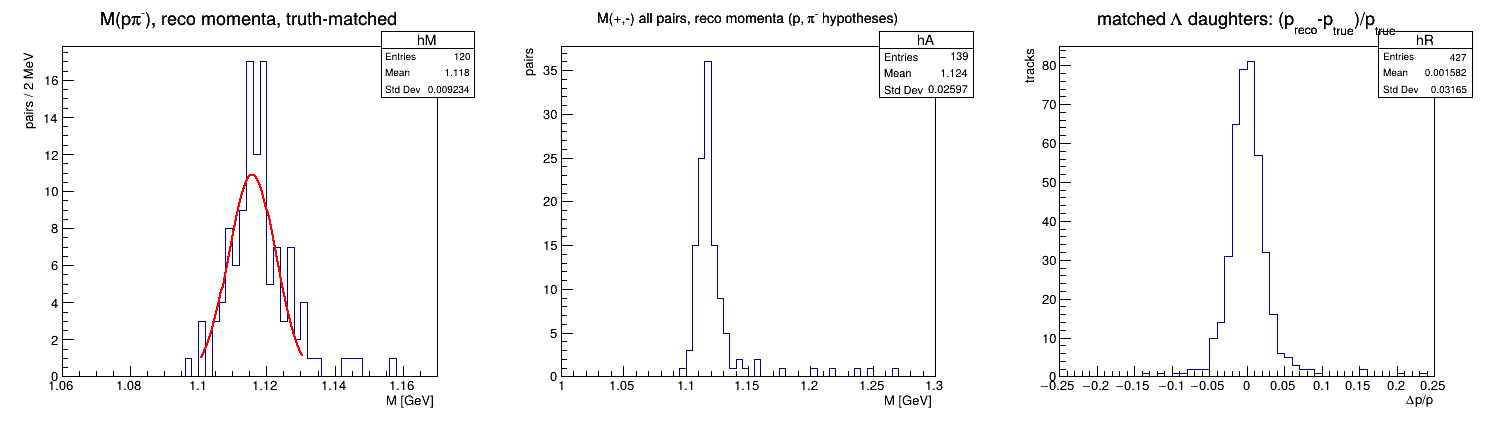
\includegraphics[width=0.85\textwidth]{06_mass/mass_reco_new_5keV.png}\\
\small new geometry, 5\,keV: truth-matched pairs (fit), all $(+,-)$ pairs, $\Delta p/p$ of the daughters\\[2mm]
\begin{tabular}{@{}lccc@{}}
\toprule
& old & new, 10\,keV & new, 5\,keV\\
\midrule
pairs (of 1000 $\Lambda$) & 150 & 101 & 120\\
mean [GeV] & $1.1177 \pm 0.0007$ & $1.1160 \pm 0.0010$ & $1.1159 \pm 0.0008$\\
$\sigma$ [MeV] & $6.3 \pm 0.6$ & $7.4 \pm 1.1$ & $6.9 \pm 1.1$\\
\bottomrule
\end{tabular}
\vspace{1mm}\\
\footnotesize PDG 1.1157\,GeV. Old geometry +2\,MeV ($\approx 3\sigma$), not understood.
\end{frame}

%-------------------------------------------------------------------------------------
\begin{frame}{$\Lambda$ mass without truth in the selection}
\begin{columns}[T]
\column{0.4\textwidth}\centering
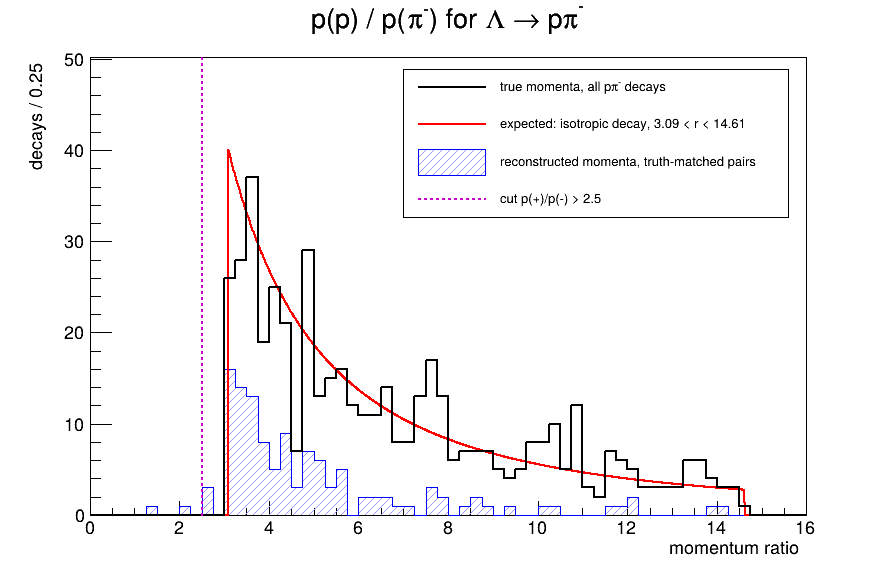
\includegraphics[width=\textwidth]{06_mass/ratio_new_5keV.png}\\
\footnotesize true ratio 3.09--14.58, as predicted; cut at 2.5 loses 2\,\% of the signal
\column{0.6\textwidth}\centering
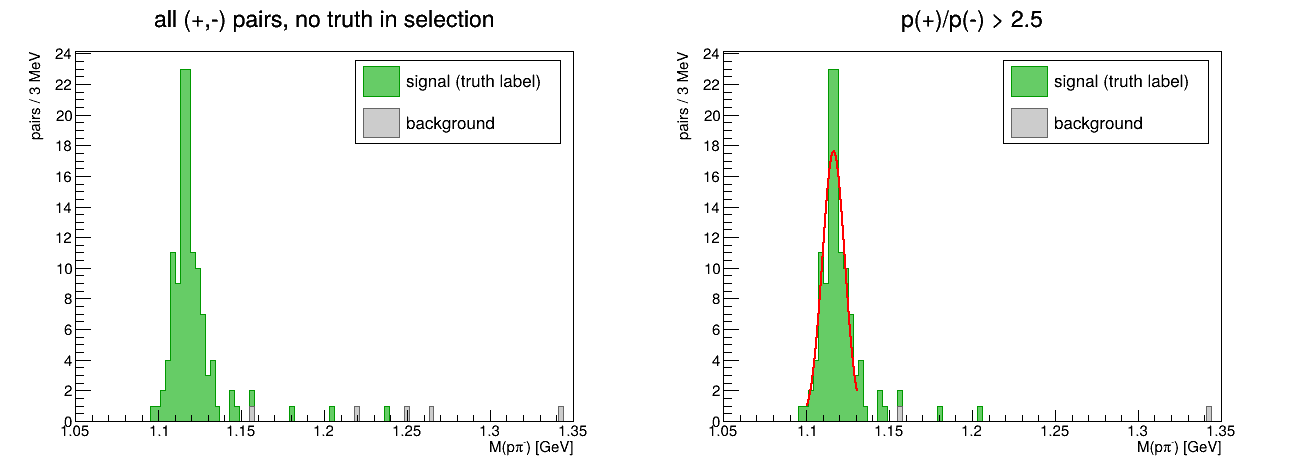
\includegraphics[width=\textwidth]{06_mass/mass_notruth_new_5keV.png}\\
\footnotesize all $(+,-)$ pairs (left), after $p(+)/p(-) > 2.5$ (right); green = signal (truth label)
\end{columns}
\vspace{2mm}
\centering\small
\begin{tabular}{@{}lccc@{}}
\toprule
& old & new, 10\,keV & new, 5\,keV\\
\midrule
after the cut: candidates / \textbf{purity} & 155 / \textbf{95\,\%} & 103 / \textbf{96\,\%} & 122 / \textbf{97\,\%}\\
$\pm 20$\,MeV window: candidates / signal & 144 / 142 & 92 / 92 & 110 / 110\\
\bottomrule
\end{tabular}
\vspace{1mm}\\
\footnotesize Tracks still truth-seeded; single-$\Lambda$ events.
\end{frame}

%-------------------------------------------------------------------------------------
\begin{frame}{Summary}
\begin{itemize}
\item B0 tracks for displaced $\Lambda$ daughters need the B0 truth seeding of \textbf{EICrecon\#2901}: 4 $\to$ 77 tracks / 100 $\Lambda$
\item Realistic B0 (\textbf{eic/epic\#1194}): $\pm 45^\circ$ $\phi$ gap on the electron side
\begin{itemize}
\item geometric acceptance 95 $\to$ 70\,\%; both daughters accepted 63 $\to$ 41\,\%
\end{itemize}
\item 50\,$\mu$m sensors need a \textbf{5\,keV threshold} (10\,keV loses 7\,\% of accepted daughters)
\item Tracking efficiency: proton 82--93\,\%, $\pi^-$ 56--61\,\%; \textbf{soft tracks ($<10$\,GeV) lost in the CKF}, not due to seed smearing
\item Both daughters reconstructed: \textbf{15\,\%} (old), \textbf{10\,\%} (new, 10\,keV), \textbf{12\,\%} (new, 5\,keV) of all $\Lambda$
\item $M(p\pi^-)$ at the PDG value, $\sigma \approx 6$--$7$\,MeV; one kinematic cut gives $\approx 97\,\%$ purity without truth
\end{itemize}
\vspace{2mm}
\textbf{Next:} CKF debugging for soft tracks; realistic seeding (EICrecon\#3028); cross-check with
EICrecon\#2926 (ChargedLambdaReconstruction); full events with backgrounds and vertexing
\end{frame}

%-------------------------------------------------------------------------------------
\appendix
\begin{frame}{Backup: reproducing the results}
\small
Repository \url{https://github.com/gadininio/eic-B0-detector}
\begin{itemize}
\item \code{macros/acceptance/}: \code{b0_geometric_acceptance.C}, \code{lambda_daughter_acceptance.C}
\item \code{macros/efficiency/}: \code{lambda_tracking_efficiency.C}, \code{lambda_acceptance_x_efficiency.C}
\item \code{macros/mass/}: truth, truth-matched, no-truth mass, momentum-ratio check
\item \code{scripts/production/lambda_sample.sh}: simulation + reconstruction (10 and 5\,keV) + copy to EOS
\item \code{scripts/make_results.sh}: every plot and number in \code{results/}
\end{itemize}
\textbf{Pitfalls}
\begin{itemize}
\item EOS not visible in eic-shell; parallel jobs in one folder race on \code{calibrations/}
\item ddsim drops hits below 1\,keV (geantinos!): \code{--filter.tracker ""}
\item EICrecon parameters need the plugin prefix (\code{tracking:}, \code{B0TRK:})
\end{itemize}
\end{frame}

\end{document}
